\subsection{Implementation}
%
Der Ablauf der Kalibrierung ist in Abbildung~\ref{fig:calibration_flowchart} in Form eine Ablaufdiagramms dargestellt. Beschrieben werden die wesentlichen Schritte. Es sind sowohl Interaktion mit der Person enthalten die die Kalibrierung durchführt, als auch die Schritte die von den beteiligten Softwarekomponenten ausgeführt werden enthalten. Es wurden im Rahmen der Arbeit zwei unterschiedliche Wege implementiert, um ein Ergebnis für die Kalibrierung zu berechnen. Diese Wege werden im Folgenden vorgestellt und die Ergebnisse miteinander verglichen. Die Präsentation der Resultate wird vor Allem dazu verwendet werden die gewählte Form der Diagramme zu erläutern. Diese werden in den Ergebnissen des komplexeren Modells ebenfalls verwendet.
%
\subsubsection{SVD}
%
Das unter \ref{sec:svd} vorgestellte Verfahren der Singular-Value-Decomposition kann dazu verwendet werden eine Lösung eines linearen Gleichungssystems zu berechnen. Das Modell, dass zur Kalibrierung verwendet wird, ist ein Gleichungssystem der Form $\mathbf{A}\mathbf{x}=\mathbf{b}$ und hat drei Gleichungen mit drei Unbekannten. Daher kann sofort eine Lösung mit dem Verfahren hergeleitet werden. Das Ergebnis eines Messaufbaus mit 3 Antennen ist in Tabelle\ref{tab:FinalCoords} und in Abbildung~\ref{fig:3dplot_coordinates} gezeigt. Die Implementation des Algorithmus stammt aus \cite{press2007numerical} und wurde für diese Arbeit angeschafft.
%
\subsubsection{CMA-ES}
Da in dieser Arbeit der CMA-ES-Algorithmus eingesetzt wird und damit ohnehin eine Implementation vorgenommen wird, kann die Kalibrierung dazu verwendet werden die Umsetzung des Algorithmus zu verifizieren. Dazu vergleichen wir das Lösung der SVD-Methode mit der des CMA-ES.\\
Das über den evolutionären Algorithmus gefundene Ergebnis gleicht dem des SVD-Verfahrens (siehe Tabelle~\ref{tab:FinalCoords}). Der SVD-Algorithmus ist um ein vielfaches effizienter\footnote{d.h. weniger Rechenzeit ist erforderlich} beim Lösen des Gleichungssystems. Die Gründe warum an dieser Stelle die Berechnung mit dem evolutionären Verfahren durchgeführt und hier dargestellt wird sind folgende:
%
\begin{enumerate}
 \item Die Komplexität ist gering, daher kann der Ablauf des evolutionären Verfahrens besser dargestellt und für später verstanden werden
 \item Der Vergleich der beiden Ergebnisse ermöglicht die Verifizierung der Implementation beider Verfahren.
\end{enumerate}
%
Dem ersten Punkt kommt im Rahmen dieser Arbeit eine besondere Stellung zu, es ist einfacher anhand dieses übersichtlichen Problems (mit nur drei Unbekannten) den Ablauf des Algorithmus sowie die Visualisierung der Ergebnisse zu veranschaulichen. Die verwendete Darstellung gleicht der, die später bei der Präsentation und Beurteilung der komplexeren Modell verwendet wird.
%
%-------------------------------------------------------------------------
\begin{figure}[H]
	\begin{center}
		\caption[Ablauf der Kalibierung]{Ablauf der Kalibierung}
		\label{fig:calibration_flowchart}
		\vspace{0.5cm}
		\begin{tikzpicture}[auto]
		\scriptsize
			\tikzstyle{decision} = [diamond, draw=black, thick, fill=black!20, text width=5em, text badly centered, inner sep=1pt]
%			
			\tikzstyle{block} = [rectangle, draw=black, thick, fill=gray!20, text width=15em, text centered, rounded corners, minimum height=4em]
%	
			\tikzstyle{line} = [draw, thick, -latex',shorten >=1pt];
			\tikzstyle{commentline} = [draw, dashed, green!50,-latex',shorten >=1pt];
%	
			\tikzstyle{cloud} = [ dotted, draw=green!50, thick, ellipse,,fill=green!20, minimum height=2em, text width= 10em, text badly centered];
%	
			\matrix [column sep=5mm,row sep=7mm]
			{
				% row 1
				& \node [block] (start) { Start }; & \\
				% row 2
				& \node [block] (setup) {Aufstellen des Kalibrierstücks}; & 
					\node [cloud] (comment1) {Gezeigt in Abbildung \ref{fig:calib_piece}}; \\
				% row 4
				& \node [block] (measure) {Vermessen der Entfernungen zu den Antennen}; & 
					\node [cloud] (comment2) {z.B. mit Laser-Entfernungsmesser, gezeigt in Abbildung \ref{fig:laser_meter}}; \\
				% row 5
				&\node [block] (writefile) {Eintragen der Vermessenen Werte in Mashinenlesbare Datei}; &\\
				% row 6
				\node (temp){}; &\node [block] (startsw) {Starte die Kalibiersoftware}; &\\
				% row 7
				&\node [block] (viewresults) {Speichern der berechneten Werte}; &\\
				% row 8				
				& \node [decision] (decide) {$\Delta \geq \Delta_{max}$}; & 
					\node [cloud] (criteria) {Ergebnisse haben eine geringe Abweichung};\\
				% row 9
				& \node [block] (stop) {Ende}; & \\
			};
			
%
%			Draw the arrows
%
			\path (decide) -| node [near start] {Nein} (temp);
			\tikzstyle{every path}=[line]
			\path (start) -- (setup);
			\path (setup) -- (measure);
			\path (measure) -- (writefile);
			\path (writefile) -- (startsw);
			\path (startsw) -- (viewresults);
			\path (viewresults) -- (decide);
			\path (decide)	-| +(-3,0)  |- (measure);
			\path (decide) -- node [midway] {Ja} (stop);
			
%			
%			draw the comments 
%
			\tikzstyle{every path}=[commentline]
			\path (criteria) -- (decide);
			\path (comment1) -- (setup);
			\path (comment2) -- (measure);
				
		\end{tikzpicture}
	\end{center}
\end{figure}
%
%-------------------------------------------------------------------------
\begin{figure}[ht!]
	\begin{center}
		\caption[Ablauf der libCalibration]{Ablauf der libCalibration}
		\label{fig:calibration_flowchart_}
		\vspace{1cm}
		\begin{tikzpicture}[auto]
		\scriptsize
			\tikzstyle{decision} = [diamond, draw=black, thick, fill=black!20, text width=5em, text badly centered, inner sep=1pt]
%			
			\tikzstyle{block} = [rectangle, draw=black, thick, fill=gray!20, text width=15em, text centered, rounded corners, minimum height=4em]
%	
			\tikzstyle{line} = [draw, thick, -latex',shorten >=1pt];
			\tikzstyle{commentline} = [draw, dashed, green!50,-latex',shorten >=1pt];
%	
			\tikzstyle{cloud} = [ dotted, draw=green!50, thick, ellipse,,fill=green!20, minimum height=2em, text width= 10em, text badly centered];
%	
			\matrix [column sep=5mm,row sep=7mm]
			{
				% row 1
				& \node [block] (start) { Start }; & \\
				% row 2
				& \node [block] (read) {Lese gemessene Werte aus CSV-Datei}; &  \\
				% row 4
				& \node [block] (read2) {Lade Geometrie des Kalibrierstücks}; & 
				 \node [cloud] (comment1) {Diagonalmatrix};\\
				% row 5
				&\node [block] (calc1) { Berechne die Matrizen für jede Antenne $\mathbf{A_k}\qquad,1 \leq k \leq |N|$ }; &  \\
				% row 6
				&\node [block] (calc2) { Berechne den Distanzvektor $\mathbf{b}$ }; &  \\			 
				% row 7
				&\node [block] (run) {Berechne die Positionen}; &
 				 \node [cloud] (comment2) {mittels SVD};\\
				% row 8
				&\node [block] (write) {Schreibe Werte}; &\\
				% row 9				
				& \node [block] (stop) {Ende}; & \\
			};
			
%
%			Draw the arrows
%
			\tikzstyle{every path}=[line]
			\path (start) -- (read);
			\path (read) -- (read2);
			\path (read2) -- (calc1);
			\path (calc1) -- (calc2);
			\path (calc2) -- (run);
			\path (run) -- (write);
			\path (write) -- (stop);
%			
%			draw the comments 
%
			\tikzstyle{every path}=[commentline]
			\path (comment1) -- (read2);
			\path (comment2) -- (run);
				
		\end{tikzpicture}
	\end{center}
\end{figure}
%\newpage
%
\subsection{Ergebnis}
Es werden nun die Ergebnisse der Kalibrierung vorgestellt. Für eine der vermessenen Antennenkonfigurationen sind in der folgenden Tabelle die Koordinaten der Antennen gezeigt. Die Visualisierung der Konfiguration zeigt die Abbildung~\ref{fig:3dplot_coordinates}.
%
\begin{table} [ht!]
	\begin{center}
		\begin{tabular}{cccccccc}
		      \textbf{Antenne} & \textbf{$x$} & \textbf{$y$} & \textbf{$z$} & \textbf{$d_{meas}$} & \textbf{$d_{result}$}& \textbf{$\epsilon_{abs}$} & \textbf{$\epsilon_{rel}$} \\
		      1 & 0.479		& -1.012	& 0.60 & 1,259 & 1,274& 0,015 & 1,14\% \\
		      2 & -0.77 	& -1.04 	& 1.34 & 1,894 & 1,872 & -0,022 & 1,19\% \\
		      3 & 1.52  	& -1.05 	& 1.37 & 2,334 & 2,307 & -0,027 & 1,15\% \\
		      4 & -0.92 	& -0.19 	& 1.32 & 1,661 & 1,628 & -0,033 & 2,01\% \\
		      5 & 1.92 		&  0.03 	& 1.39 & 2,399 & 2,375 & -0,024 & 1,01\% \\
		      6 & -0.55 	&  1.09 	& 1.43 & 1,851 & 1,887 & 0,036 & 1,93\% \\
		      7 & 1.06 		&  1.07 	& 1.35 & 2,055 & 2,031 & -0,024 & 1,19\% \\
		      8 & 0.45 		&  1.35 	& 0.67 & 1,574 & 1,578 & 0,004 & 0,26\% \\					
%
		\end{tabular}
		\caption[Finale Antennen Koordinaten]{Tabelle der finalen Antennenkoordinaten [m], berechnet mit dem in dieser Arbeit entwickelten Modell und dem SVD-Verfahren, die Ergebnisse wurden auf zwei Nachkommastellen gerundet und sind identisch für beide Methoden. Die Spalte $d_{result}$ enthält die von der Berechnung gefundenen Distanz vom Referenzpunkt zur Antenne. Die Spalte $d_{meas}$ zeigt die gemessenen Werte. Die $\epsilon$-Spalten zeigen die Abweichung.}
		\label{tab:FinalCoords}
	\end{center}
\end{table}
%
Eine Berechnung mit dem evolutionären Verfahren dauerte ca. $170$~ms mit dem SVD-verfahren wurde eine Lösung und $\le 1$~ms gefunden. Für die in der Praxis eingesetzte Software wird es eine Implementation der Kalibrierung mit dem SVD-Verfahren geben. Das Ergebnis der mit dieser Variante berechnete Verfahren wird bei Bedarf mit einer Lösung des evolutionären Verfahrens verglichen. Das ermöglicht eine Build-In Verifikation der Kalibrierung.\\

\subsubsection{Visualisierung der Ergebnisse}
Für die in den folgenden Abbildungen präsentierten Ergebnisse wurden insgesamt $100$ Durchläufe des Algorithmus erstellt. Die Ergebnisse wurden mit einem vom Algorithmus selbst erstellten $\mu$ und $\lambda$ gefunden. In Abbildung~\ref{fig:Final_Calibration_Ant0_ES-boxes} wird eine statistische Auswertung der Ergebnisse gezeigt. In jedem Plot werden die Endwerte der Lösungen in einem sog. Boxplot gezeigt. Dabei wird die Verteilung mit Hilfe von Boxen dargestellt. Die Fähnchen der Boxen, stellen die maximal- bzw. minimal-Werte dar. Die Größe der Boxen enthält das obere und untere Quartil der Daten, der horizontale Strich in der Box zeigt den Mittelwert der Daten. Ausreißer\footnote{Hier Werte die den $2$-Fachen Wert des oberen- bzw. unteren-Quartils aufweisen} in den Daten werden durch Punkte abseits der Box dargestellt.\\
%

Die Abbildung.~\ref{fig:Final_Calibration_Ant0_ES-boxes} zeigt den Verlauf der drei Objektvariablen ($x,y,z$-Koordinaten) sowie die Entwicklung der Fitness und des mittleren Sigmas. Als Darstellungsart wird der Linienplot verwendet und die Verläufe einzelner Lösungen überlagern sich in diesem Plot. Das Abbruchkriterium war eine Fitness von $\leq 10^{-25}$. Für Darstellungszwecke wurde die $x$-Achse nach $500$ Werten beschränkt, daher erreicht der Fitness-Plot diesen Wert in der Abbildung nicht. Der Verlauf ist typisch für den verwendeten Algorithmus. Deutlich zu erkennen ist eine Verbesserung des Ergebnisses mit steigender Zahl der Generationen. Der Verlauf der Variablen ist immer für den erfolgreichsten Nachkommen einer Generation dargestellt.\\
%

Abbildung~\ref{fig:Final_Calibration_Ant0_ES-Scatter} ist ein Scatter-Plot. Die Objektvariablen werden hier gegeneinander aufgetragen. Auf der Diagonalen befinden sich stets die Variable gegen sich selbst aufgetragen, daher zeigt sich dort immer eine Linie, bei streuenden Ergebnissen, bzw. ein einzelner Punkt, sollten die Ergebnisse nicht streuen. Der Plot ist praktisch um die Implementation des Algorithmus zu verifizieren. Er lässt Rückschlüsse auf Abhängigkeiten und Einflüsse der Objektvariablen zu. So können die Ergebnisse mit den Erwartungen an die Verläufe verglichen werden.\\
%
%---------------------------------------------------------------
%
\begin{figure}[!ht]
  \begin{center}
   \caption[Box-Plot der Endergebnisse der Kalibierung]{Boxplot des Kalibierergebnis aus $100$ Durchläufen. Im oberen Plot der sind die x,y,z-Koordinaten gezeigt, diese landen in allen Durchläufen auf dem selben Ergebnis. Was nicht verwundert, das Problem ist eines der Art drei Gleichungen und drei Unbekannte. Die Streuung der Lösung zeigt sich in der Breite der Linien. Die unteren vier Plots zeigen die Anzahl der Evaluationen der Fitness-Funktion, den finalen Funktionswert, das Sigma für die Variablen, die Entfernung zum Referenzpunkt (v.l.n.r.). Das Ergebnis sind die Koordinaten für Antenne 1}
    \label{fig:Final_Calibration_Ant0_ES-boxes}
    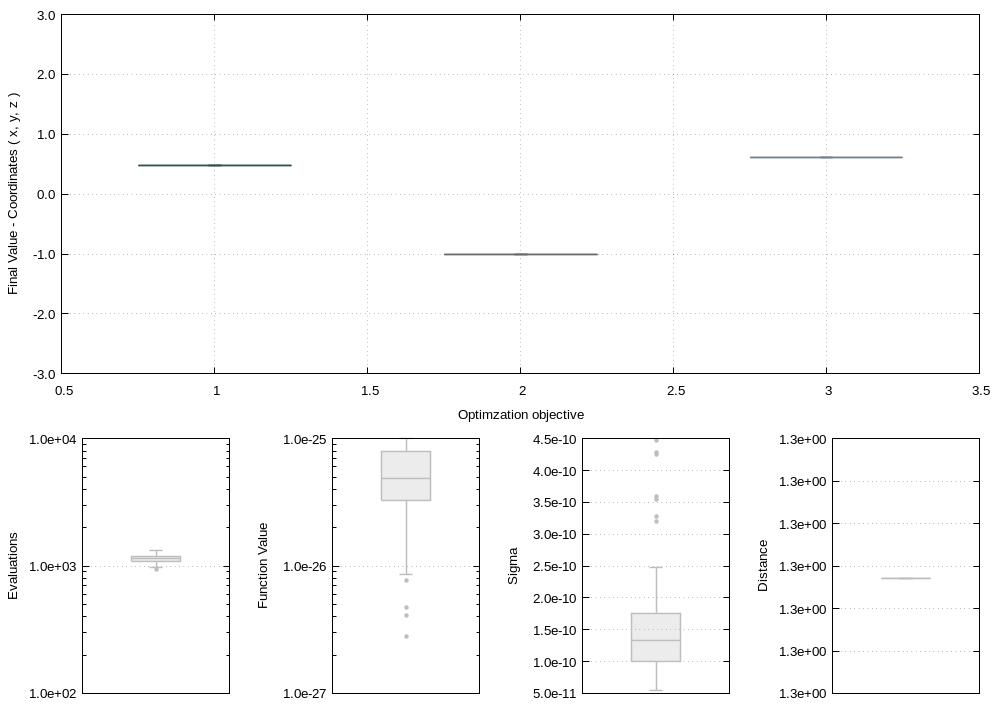
\includegraphics[width=0.9\textwidth]{img/calibration/calibration_ant0-boxes.png}
  \end{center}
 
%
\end{figure}
%
%---------------------------------------------------------------
%
\begin{figure}[!ht]
  \begin{center}
    \caption[Linien-Plot der Endergebnisse der Kalibierung]{Zu erkennen ist, das nach ca. 300 Evaluationen der Zielfunktion keine großen Änderungen der Variablen zu erkennen sind. Bis zum erreichen des Abbruchkriteriums (Function Value $\leq10^{-25}$) werden noch ca 400 Evaluationen benötigt, vgl. korrespondierender Boxplot.}
    \label{fig:Final_Calibration_Ant0_ES-Lines}  
    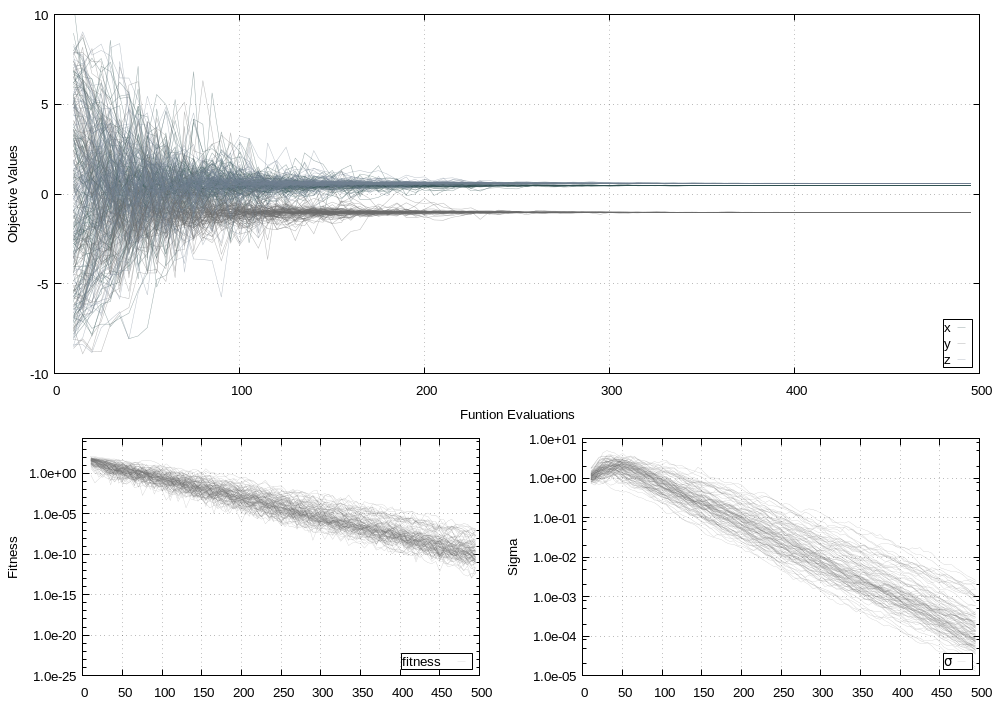
\includegraphics[width=0.9\textwidth]{img/calibration/calibration_ant0-lines.png}
  \end{center}
%  
\end{figure}
%---------------------------------------------------------------
%
\begin{figure}[!ht]
  \begin{center}
  
    \caption[Kalibierung Scatter-Plot]{Scatter-Plot der Ergebnisse der evolutionären Kalibrierung. Die Endergebnisse streuen in keiner Dimension, das wird aus dieser Darstellung deutlich. Wenngleich der Plot etwas langweilig anmutet.}
    \label{fig:Final_Calibration_Ant0_ES-Scatter}  
    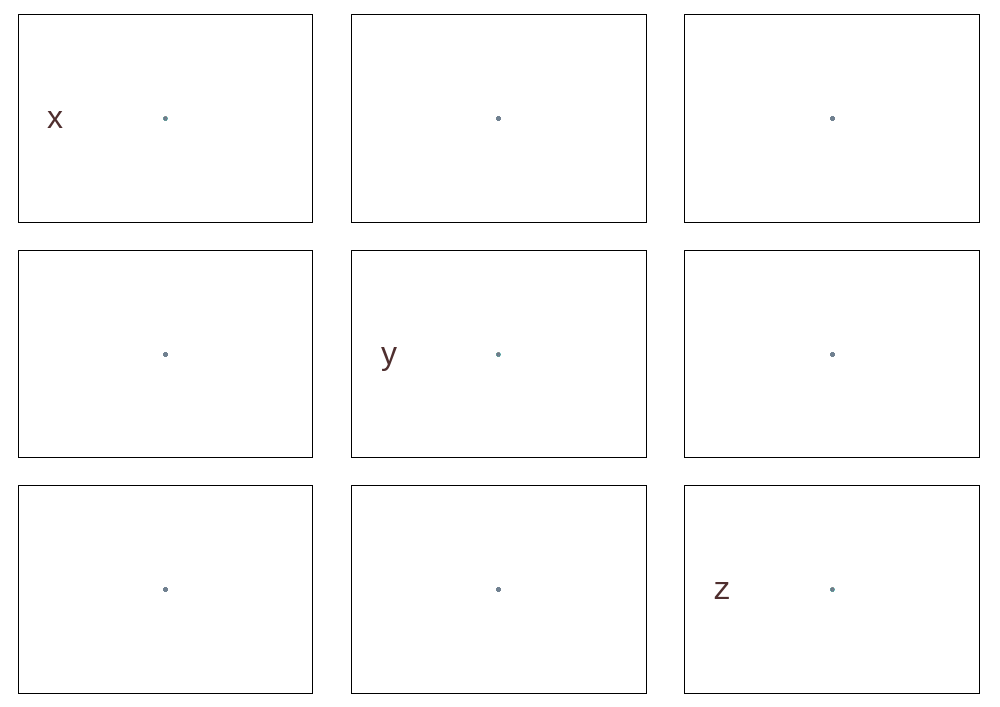
\includegraphics[width=0.9\textwidth]{img/calibration/calibration_ant0-scatter.png}
  \end{center}
%  
\end{figure}
%---------------------------------------------------------------
%
\begin{figure}[!ht]
     \centering
     \begin{subfigure}[t]{0.45\textwidth}
             \centering
             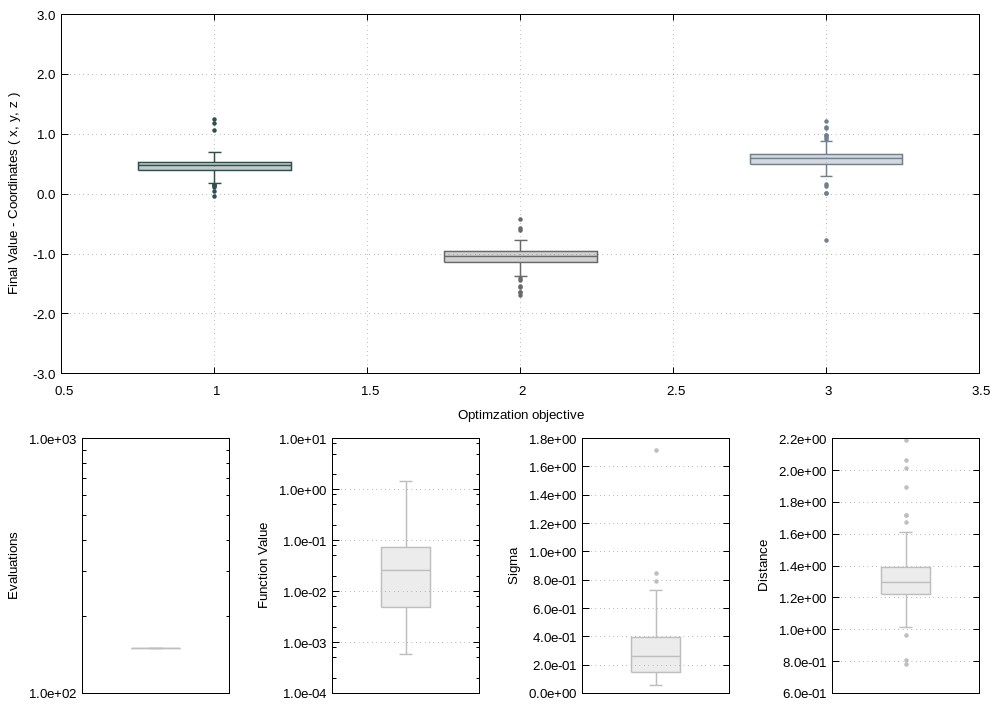
\includegraphics[width=\textwidth]{img/calibration/aborted_calibration_ant0-boxes.png}
             \caption{Statistisch verteilte Endwerte für die Koordinaten der Kalibrierung.}
             \label{fig:abortedFinal_Calibration_Ant0_ES-boxes}
     \end{subfigure}
%
\qquad         
%
     \begin{subfigure}[t]{0.45\textwidth}
             \centering
             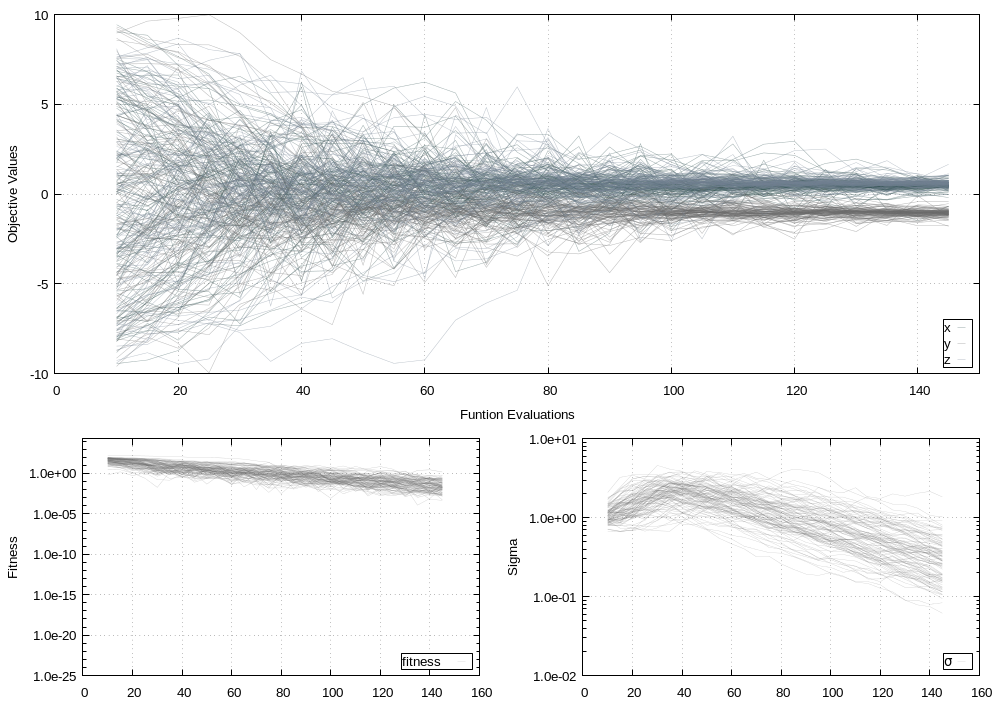
\includegraphics[width=\textwidth]{img/calibration/aborted_calibration_ant0-lines.png}
             \caption{Linienplot der bei $140$ Evaluationen abgebrochenen Verläufe. Gut zu sehen ist der Verlauf der Objektvariablen, die sich von Generation zu Generation dem realen Wert nähern}
             \label{fig:abortedFinal_Calibration_Ant0_ES-Lines}
     \end{subfigure}
%
\\
%
     \begin{subfigure}[t]{0.4\textwidth}
             \centering
             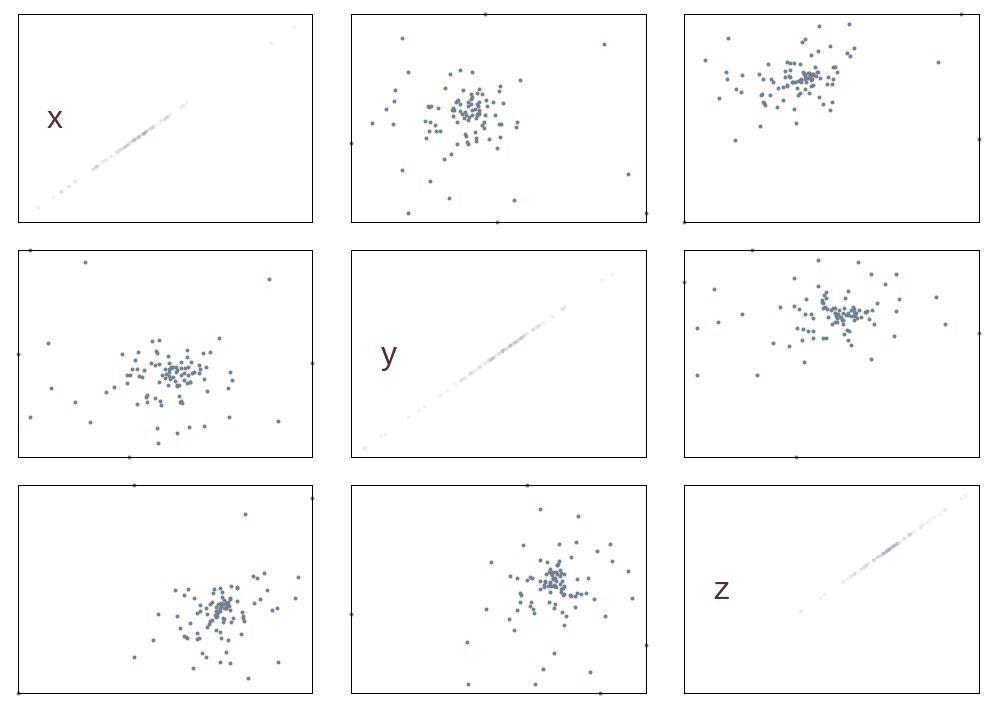
\includegraphics[width=\textwidth]{img/calibration/aborted_calibration_ant0-scatter.png}
             \caption{Statistische Streuung um einen Mittelwert. So in etwa kann man die Lösungen der Komplexen Probleme erwarten.}
             \label{fig:abortedFinal_Calibration_Ant0_ES-Scatter}
     \end{subfigure}
%
     \caption[Statistisch verteilte Ergebnisse der Kalibrierung mittels ES]{Analog zu der Abbildungen~\ref        {fig:abortedFinal_Calibration_Ant0_ES-Lines}, \ref{fig:abortedFinal_Calibration_Ant0_ES-boxes} und \ref{fig:abortedFinal_Calibration_Ant0_ES-Scatter} zeigen die Plots die gleichen Darstellungen. Hier gezeigt wird wie sich eine statistische Verteilung in den Plots manifestieren würde. Um das zu demonstrieren wurde das Abbruchkriterium auf lediglich $150$ Evaluationen der Zielfunktion eingestellt. Zu diesem Zeitpunkt können die Objektvariablen bereits einen passablen Wert erreicht haben oder noch abweichende Werte aufweisen (vgl. \ref{fig:Final_Calibration_Ant0_ES-Lines}).}
     \label{fig::abortedFinal_Calibration_Ant0_ES}
\end{figure}
%
\begin{figure}[ht!]
         \centering
         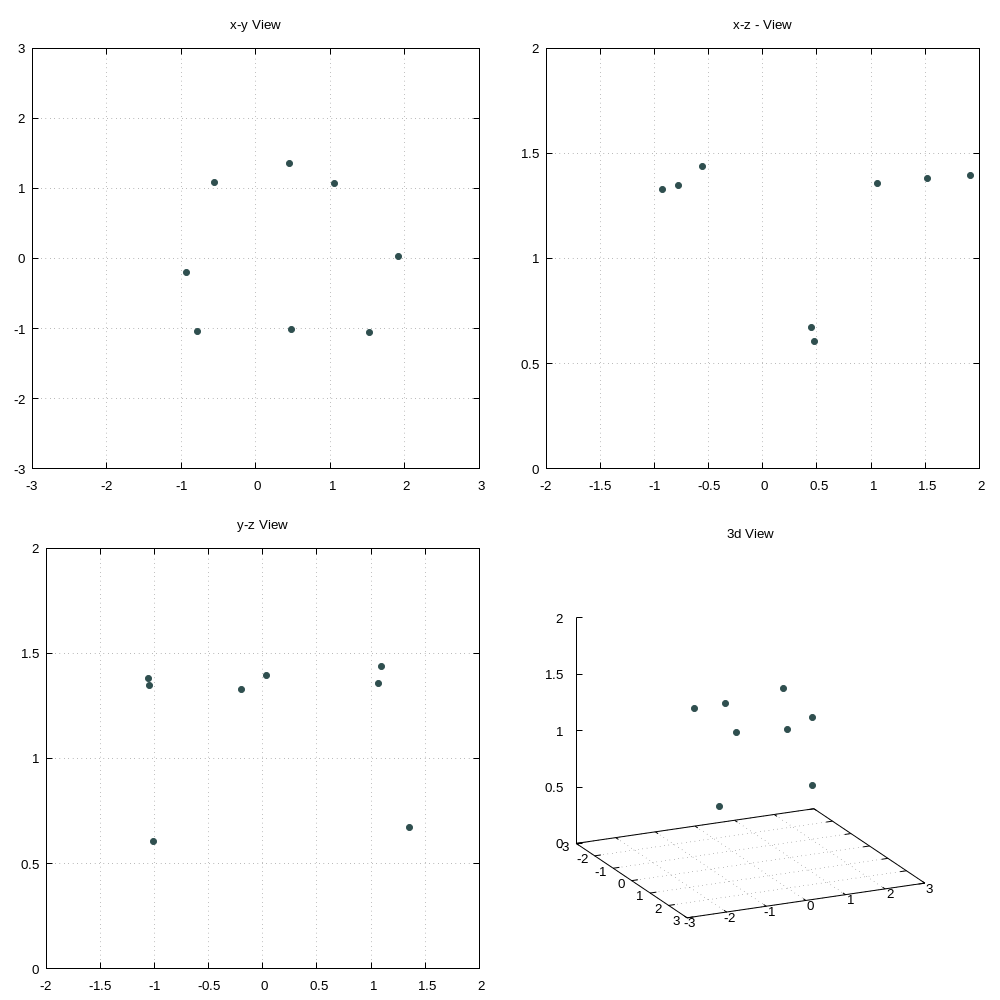
\includegraphics[width=0.7\textwidth]{img/calibration/calibration_results.png}
         \caption[Visualisierung des Kalibrierendergebnis]{Visualisierung des Kalibrierendergebnis. Abgebildet sind die gefundenen Antennenkoordinaten (Punkte) in drei Raumansichten. Die zusätzliche, dreidimensionale  Ansicht dient der Überischt. Das Ergebnis und die reale Anordnung decken sich sehr gut. }
         \label{fig:3dplot_coordinates}
%
\end{figure}
%
\begin{figure}[ht!]
         \centering
         \caption[Kalibrierwerkzeuge]{Werkzeuge die bei der Kalibrierung verwendet werden.}
         \begin{subfigure}[t]{0.4\textwidth}
                 \centering
                 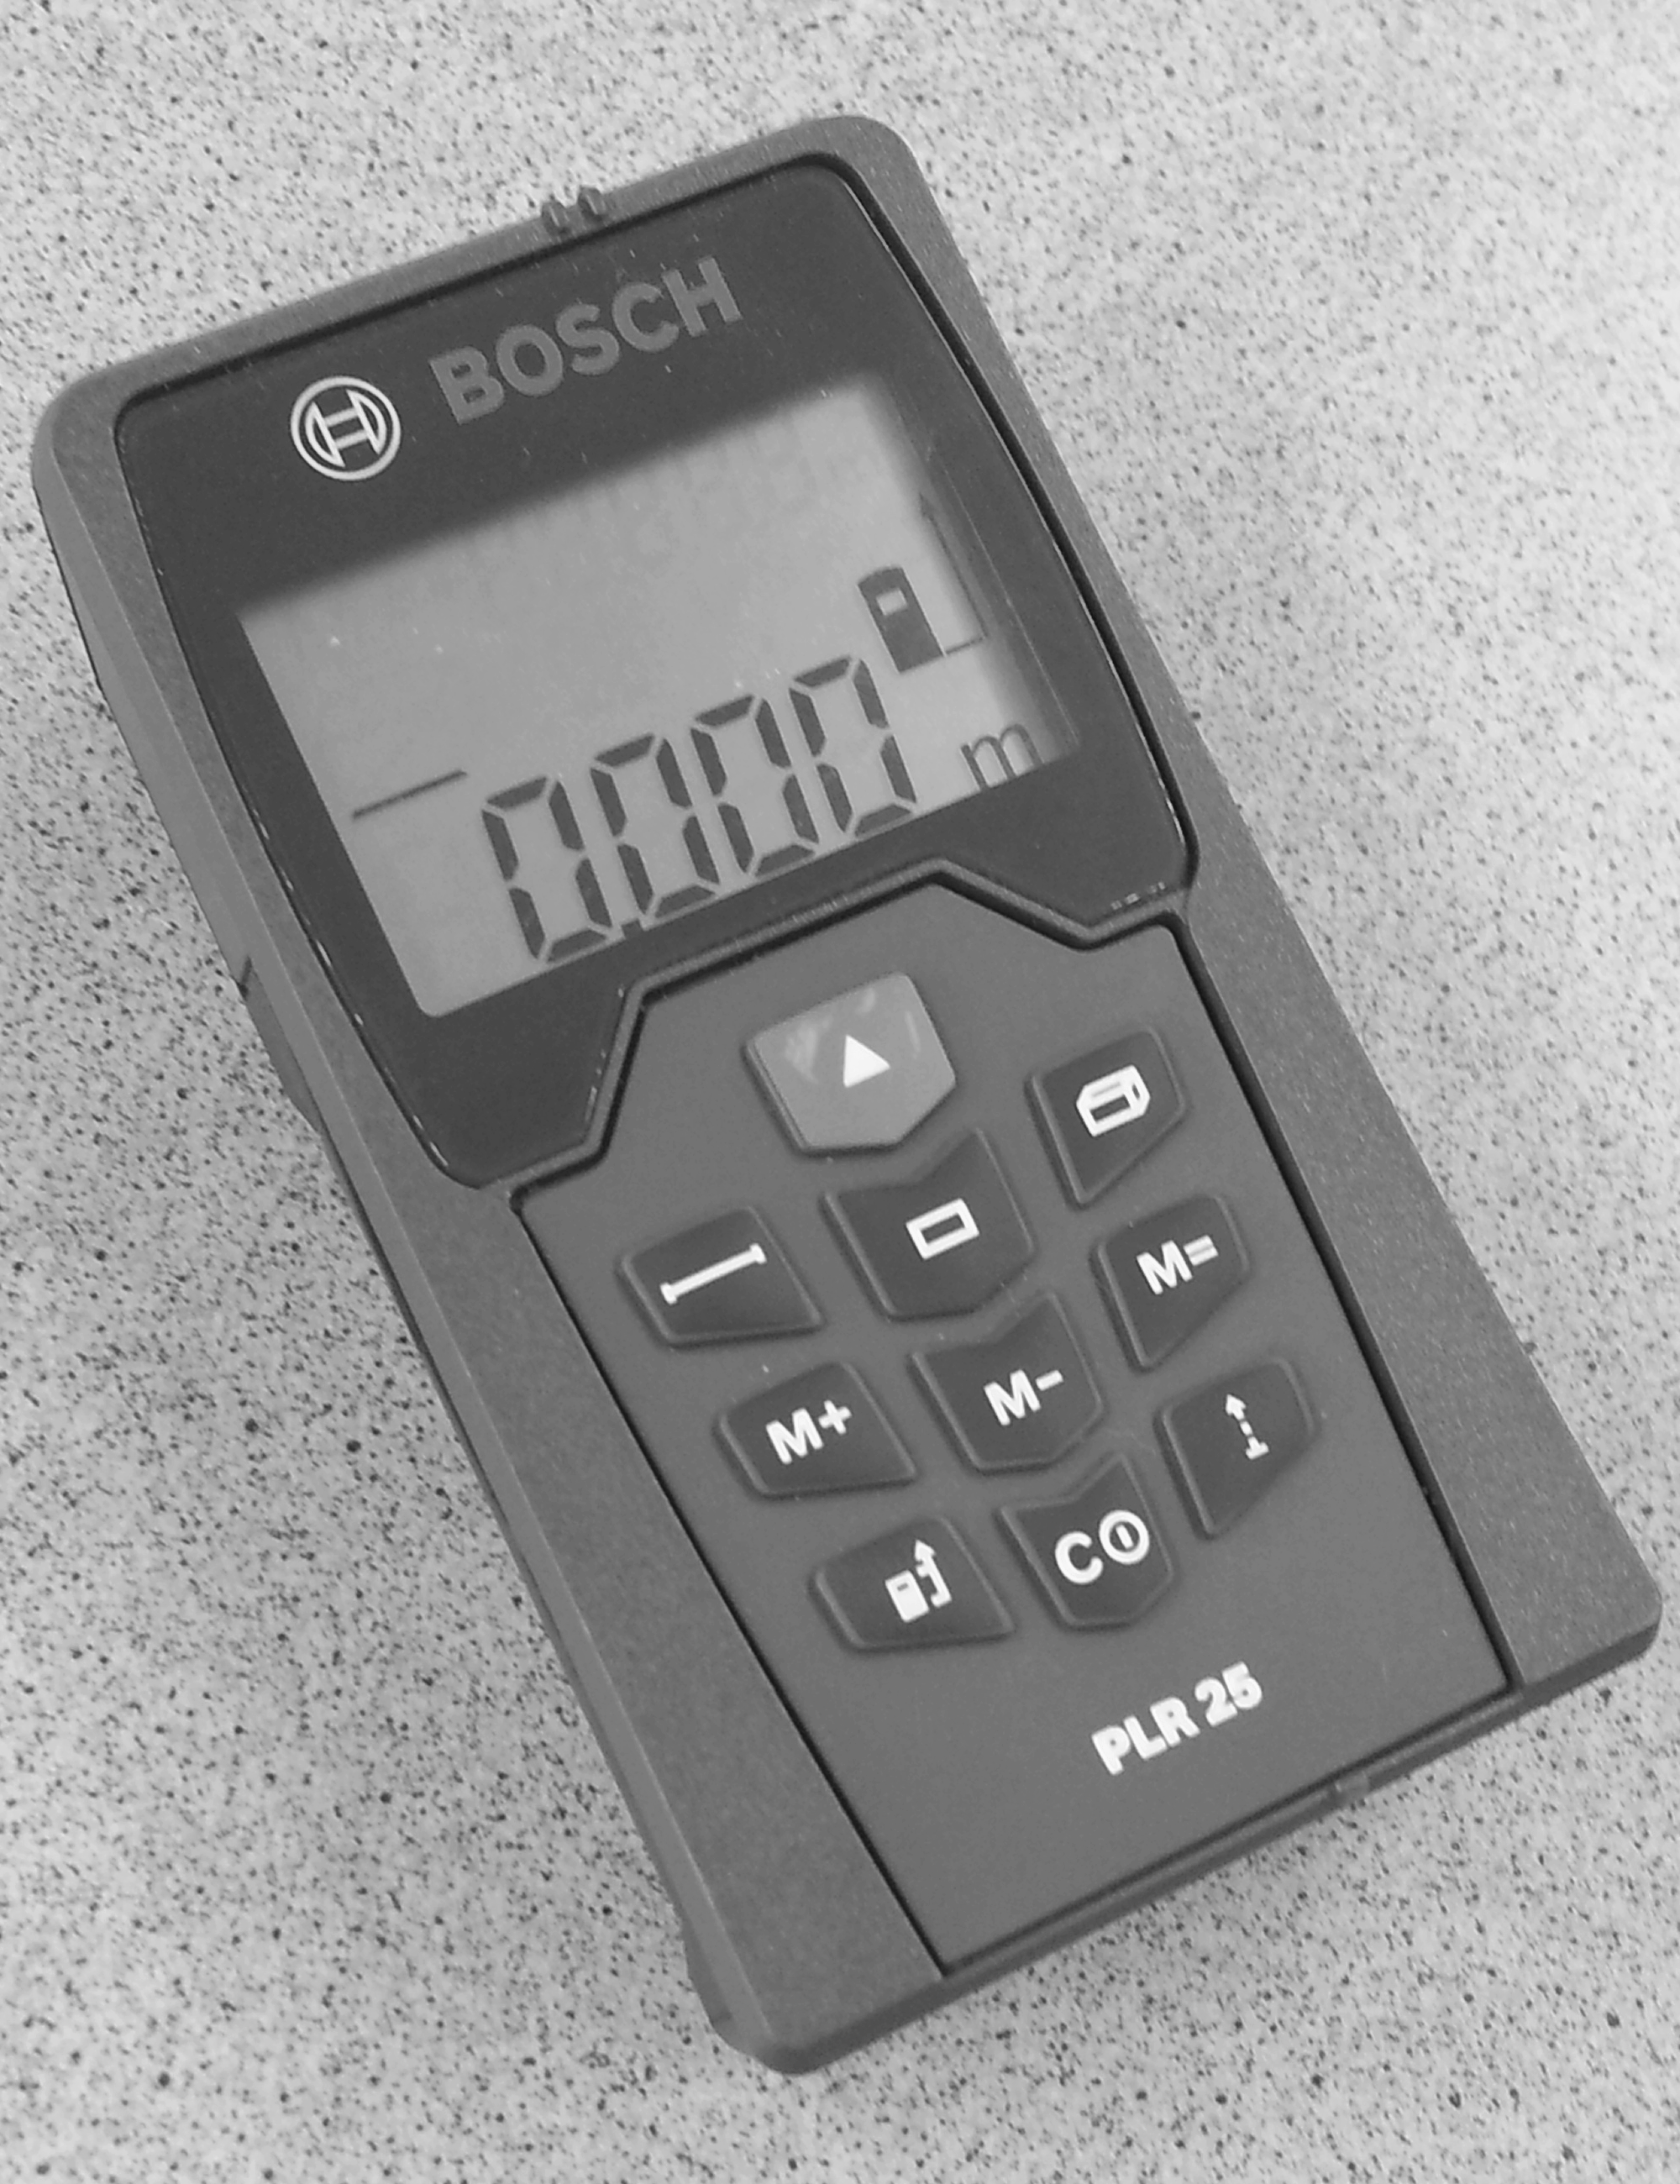
\includegraphics[width=\textwidth]{img/Lasermeter.png}
                 \caption{Laser Distanzmesser}
                 \label{fig:laser_meter}
         \end{subfigure}
%
\qquad         
%
         \begin{subfigure}[t]{0.4\textwidth}
                 \centering
                 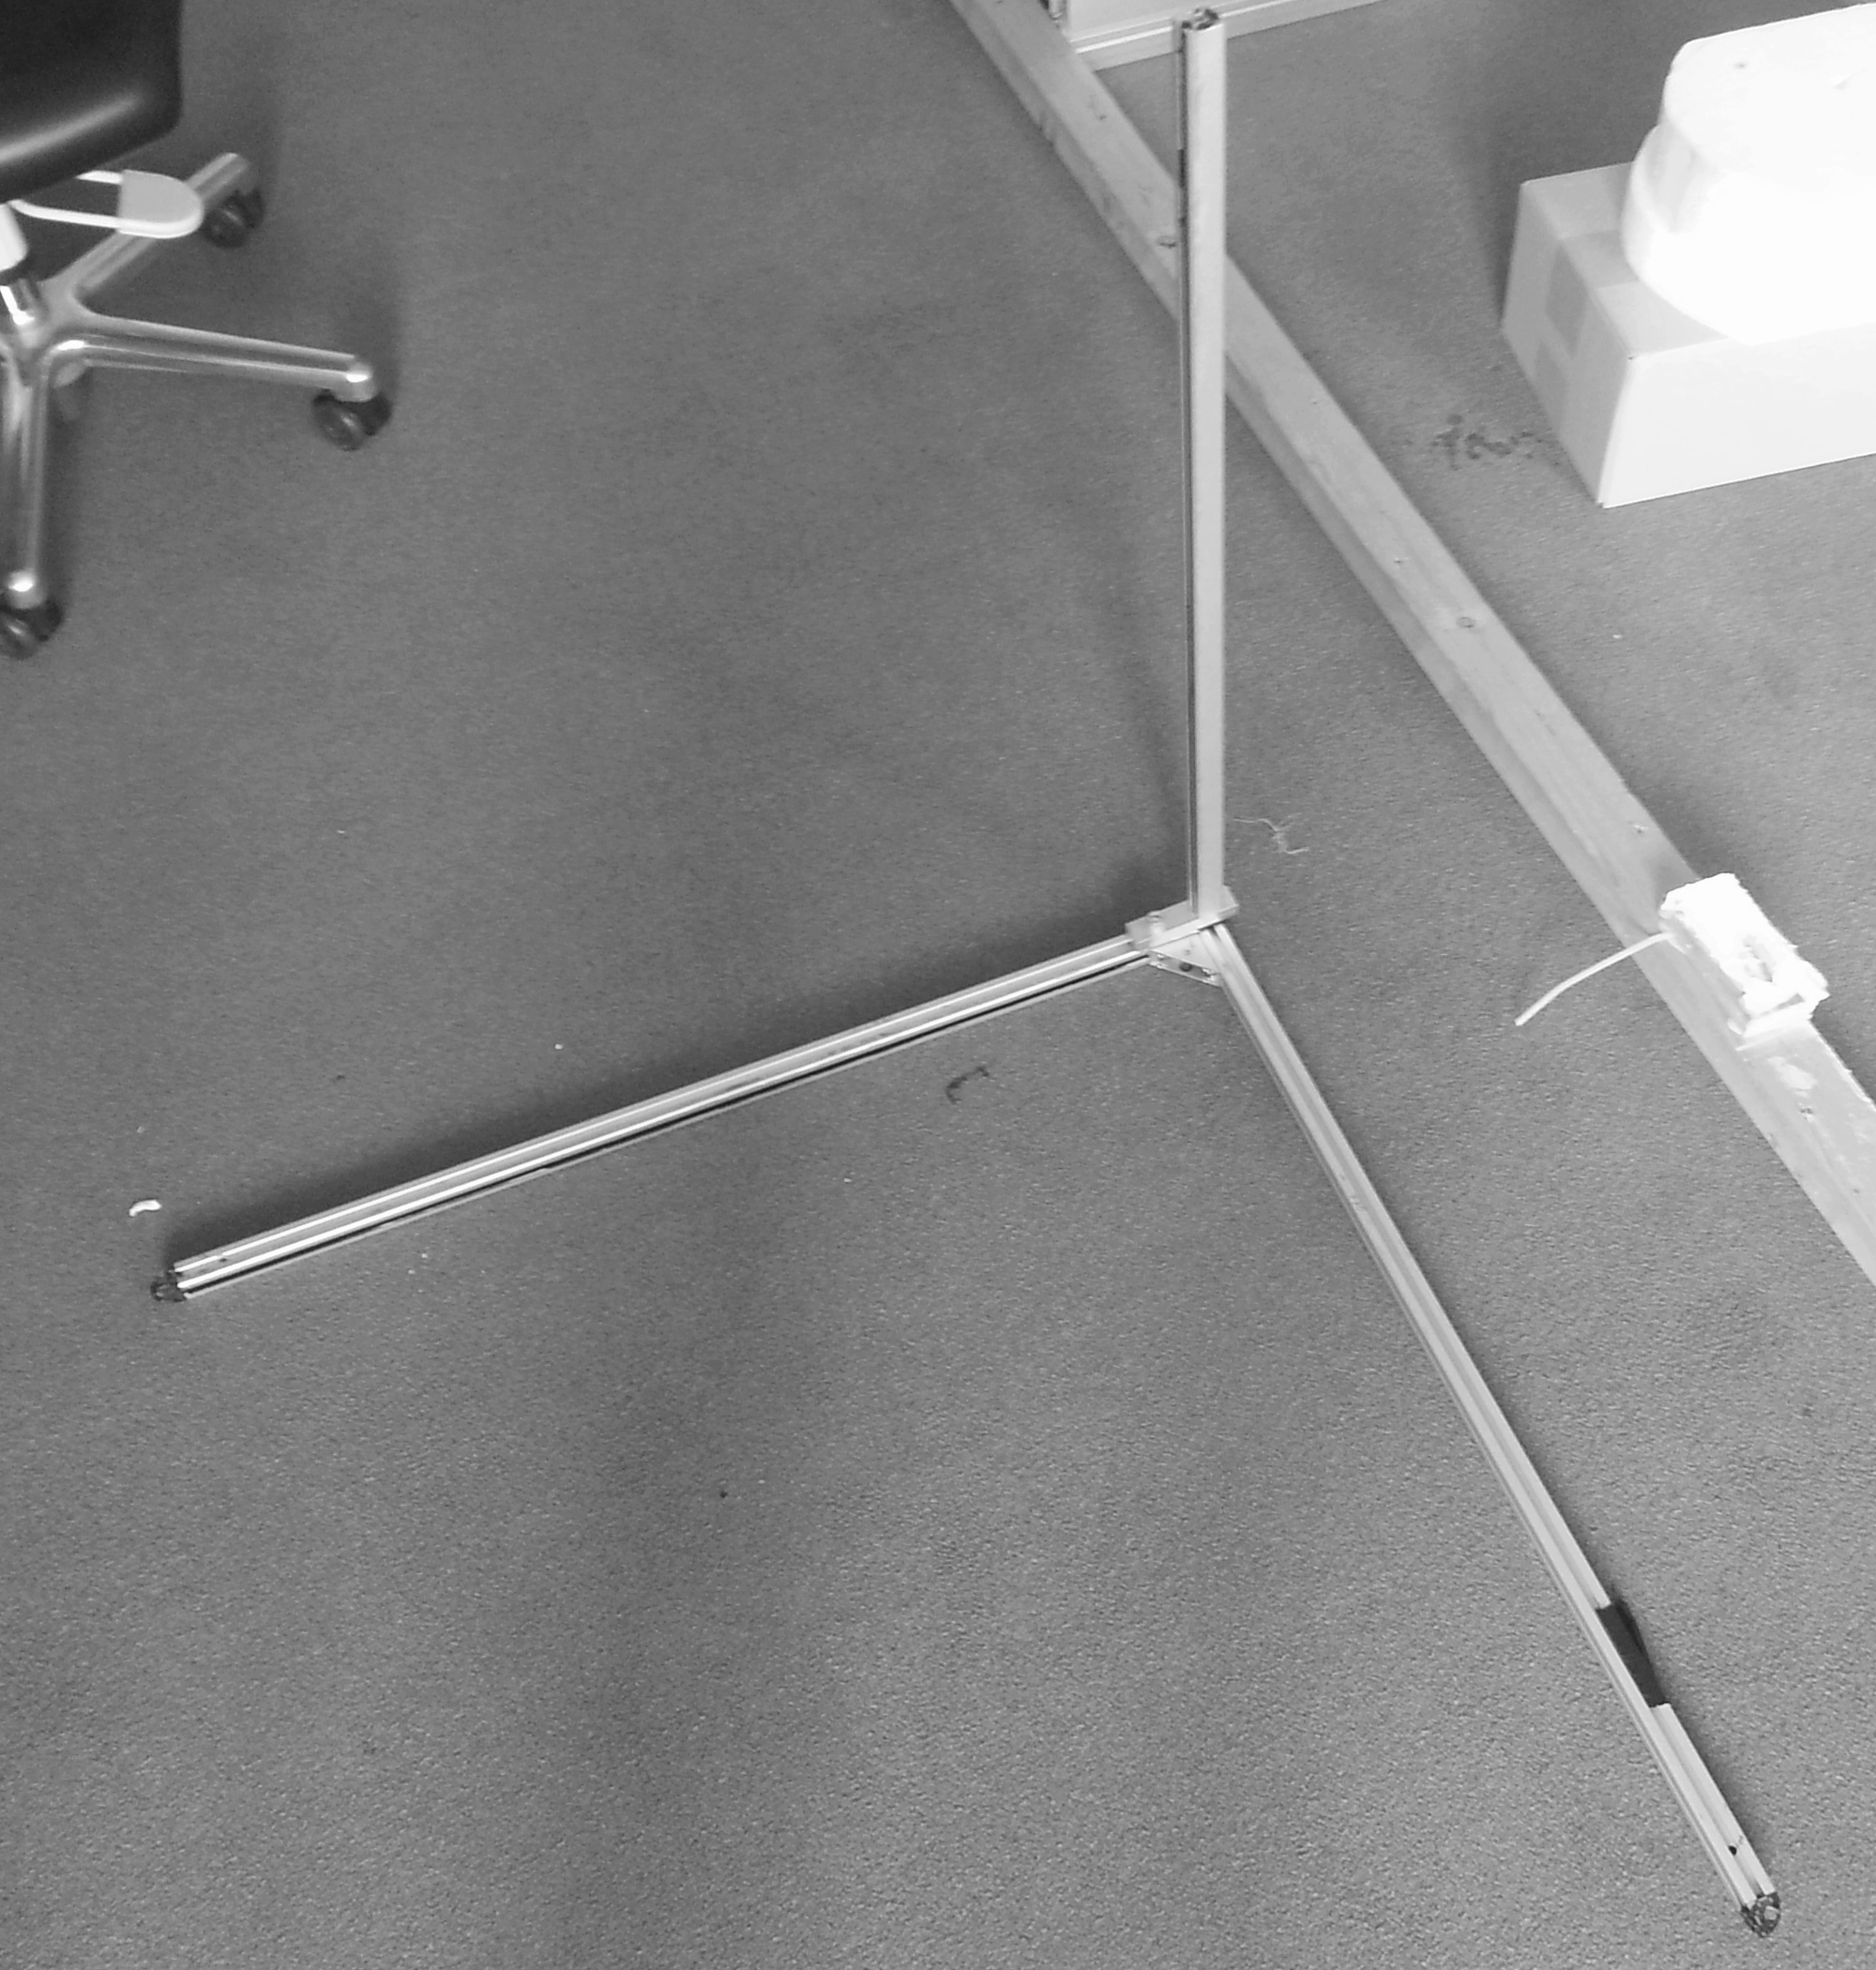
\includegraphics[width=\textwidth]{img/Calibration_Phantom.png}
                 \caption{Kalibrierstück mit vier Messpositionen. }
                 \label{fig:calib_piece}
         \end{subfigure}
         \label{fig:Calibration_Tools}
\end{figure}
 